\documentclass[aspectratio=169]{beamer}



% OPCIONES DE BEAMER

\definecolor{Maroon}{cmyk}{0, 0.87, 0.88, 0.1}
\definecolor{teal}{rgb}{0.0, 0.45, 0.45}

\usetheme[block=fill,numbering=fraction,, subsectionpage=progressbar, titleformat section=smallcaps]{metropolis}
\setbeamertemplate{blocks}[rounded][shadow=false]
\setbeamertemplate{frametitle continuation}[roman]
\setbeamertemplate{section in toc}[balls numbered]
\setbeamertemplate{subsection in toc}[subsections unnumbered]
%\setsansfont[BviejoFont={Fira Sans SemiBold}]{Fira Sans Book}  % Increase font weigth
\widowpenalties 1 10000
\raggedbottom

% COLORES
\setbeamercolor{palette primary}{bg=teal}
\setbeamercolor{progress bar}{use=Maroon, fg=Maroon}

% PAQUETES
\usepackage{bm}
\usepackage{xcolor}
\colorlet{shadecolor}{blue!15}
\usepackage{framed}
\usepackage{amsthm}
\usepackage[utf8]{inputenc}
\usepackage[english]{babel}
\usepackage{subfig}
\usepackage{graphicx}
\usepackage{minted}
\usepackage{ upgreek }
\usepackage{multirow}
\usepackage{makecell}


% Macros
\newcommand{\bx}{\bm{x}}
\newcommand{\bX}{\bm{X}}
\newcommand{\bw}{\bm{w}}
\newcommand{\bW}{\bm{W}}
\newcommand{\bz}{\bm{z}}
\newcommand{\bZ}{\bm{Z}}
\newcommand{\bv}{\bm{v}}
\newcommand{\bV}{\bm{V}}
\newcommand{\bH}{\bm{H}}
\newcommand{\bh}{\bm{h}}
\newcommand{\bSigma}{\bm{\Sigma}}
\newcommand{\bpi}{\bm{\pi}}
\newcommand{\bLambda}{\bm{\Lambda}}
\newcommand{\bmu}{\bm{\mu}}
\newcommand{\btheta}{\bm{\theta}}
\newcommand{\bnu}{\bm{\nu}}
\DeclareMathOperator*{\argmax}{arg\,max}
\DeclareMathOperator*{\argmin}{arg\,min}
\newcommand\E[2]{\mathbb{E}_{#1}\left[#2\right]}
\newcommand\KL[2]{D_{KL}\Big(#1 \bigm|\bigm| #2\Big)}
\newcommand{\bigCI}{\mathrel{\text{\scalebox{1.07}{$\perp\mkern-10mu\perp$}}}}
\newcommand{\bigCD}{\centernot{\bigCI}}
\newcommand{\X}{\mathcal{X}}
\newcommand{\R}{\mathbb{R}}
\usepackage{pgfplots}
%bib

%\bibliography{bibliography.bib}\
%\nocite{*}

\newcommand{\norm}[1]{\left\lVert#1\right\rVert}
\newcommand{\abs}[1]{\left\lvert#1\right\rvert}
\newcommand{\ps}{x^+}
\newcommand{\ns}{x^-}


% TikZ
\usepackage{tikz}

\usepackage{arydshln}
\usepackage{natbib}



\AtBeginSubsection{}

\captionsetup[subfloat]{labelformat=empty}

\newtheorem{defi}{Definition}
\newtheorem{prop}{Proposición}
\newtheorem{nth}{Teorema}
\newtheorem{cor}{Corolario}
\newtheorem{ex}{Example}

\definecolor{studentbrown}{RGB}{124,71,50}
\AtBeginEnvironment{ex}{
    \setbeamercolor{block title}{use=example text,fg=white,bg=example text.fg!75!black}
    \setbeamercolor{block body}{parent=normal text,use=block title example,bg=block title example.bg!10!bg}
}

\usetikzlibrary{arrows.meta,
chains,
positioning}

\newcommand\Fontvi{\fontsize{8}{7.2}\selectfont}

\title{Triplet loss functions in speaker recognition systems}
\date{\today}
\author{Francisco Javier Sáez Maldonado}
\institute{Máster en Ciencia de Datos \\\\\\ \emph{Escuela Politécnica Superior} \\ \emph{Universidad Autónoma de Madrid}}

\usepackage[absolute,overlay]{textpos}


\begin{document}
\setbeamercolor{background canvas}{bg=white}
\maketitle


\begin{frame}{Introduction}

  \begin{itemize}
    \item \textbf{Task}: Speaker Recognition
          \begin{itemize}
            \item 'Closed-set' vs 'Open-set'
          \end{itemize}
          \pause
    \item \textbf{Data}: VoxCeleb challenge dataset.
  \end{itemize}
\end{frame}

\begin{frame}{Original Paper}
  \begin{figure}
    \centering
    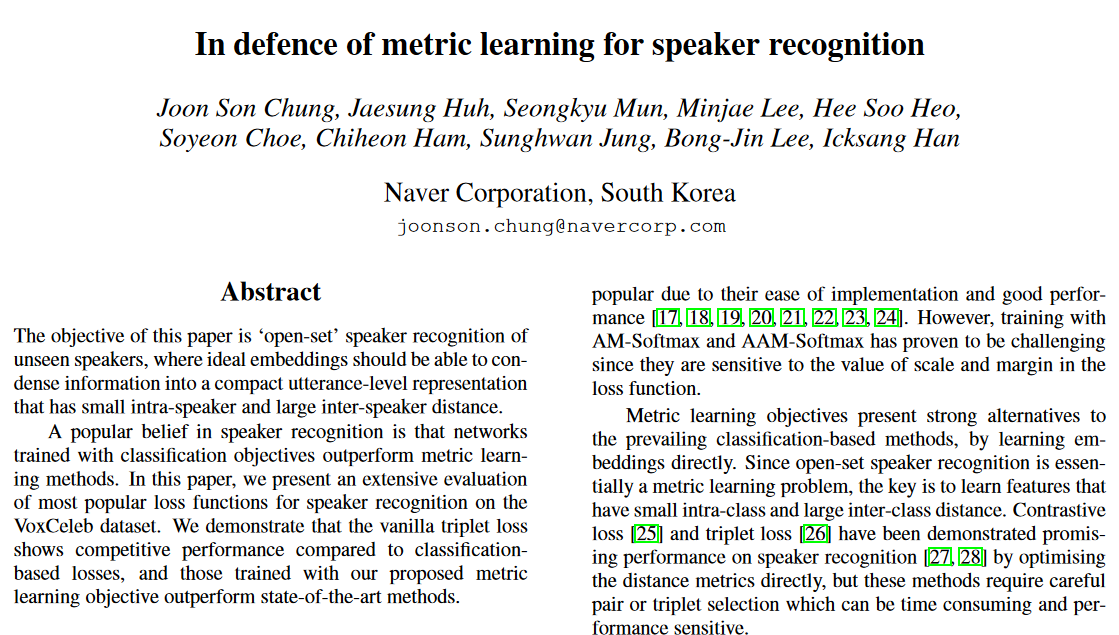
\includegraphics[scale=0.5]{Figures/paper.png}
  \end{figure}
\end{frame}


\begin{frame}{Softmax is not enough}
  \begin{itemize}
    \item \textbf{Softmax:} \(\displaystyle L_S = - \frac{1}{N} \sum_{i=1}^N \log \frac{e^{\mathbf{W}^T_{y_i} x_i + b_{y_i}}}{\sum_{j=1}^C e^{\mathbf{W}^T_j x_i + b_j} }\)
  \end{itemize}
  \pause
  \begin{figure}
    \centering
    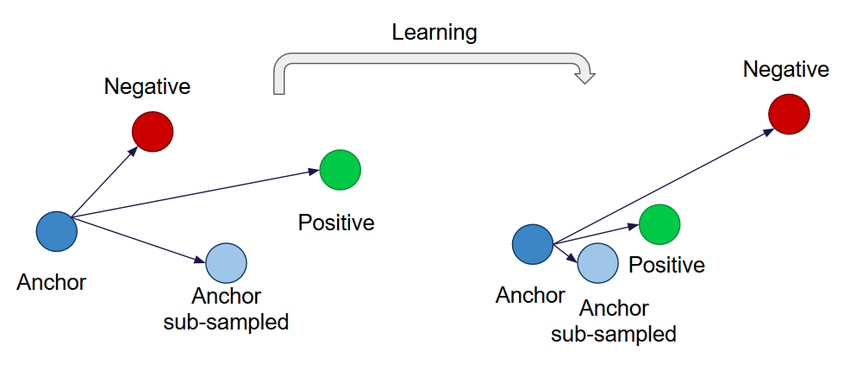
\includegraphics[scale=0.4]{Figures/TripletLoss.png}
  \end{figure}
\end{frame}




\section{Tools}
\begin{frame}{Conclusions}

  \begin{itemize}
    \item Usage of two general machine learning techniques applied to natural language processing.
    \item Applying this method has a similar effect to regularization.
    \item Results are promising in Language modeling, but not so much in Neural Machine Translation.
  \end{itemize}
\end{frame}

\appendix

\begin{frame}[noframenumbering,standout]
  Thank you for your \textcolor{brown}{attention}.
\end{frame}


\begin{frame}[noframenumbering]

  \vspace{0.5cm}
  \bibliographystyle{dinat}
  \bibliography{bibliography.bib}

\end{frame}



\end{document}
